\documentclass{article}
\usepackage{graphicx}
\usepackage[margin=1.5cm]{geometry}
\usepackage{amsmath}
\usepackage{hyperref}

\begin{document}

\title{Warm Up: The Concept of a Force}
\author{Prof. Jordan C. Hanson}

\maketitle

\begin{figure}
\centering
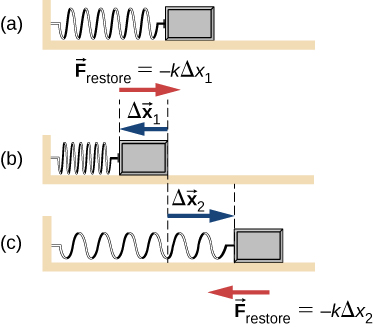
\includegraphics[width=0.33\textwidth]{figures/spring.jpeg}
\caption{\label{fig:1} A spring exerts a force on a mass when compressed or stretched.}
\end{figure}

\section{Memory Bank}

\begin{enumerate}
\item $\vec{F} = - k \Delta \vec{x}$ ... The ``force'' exerted by a spring compressed or stretched by a displacement $\Delta \vec{x}$.
\end{enumerate}

\section{Force and Springs}

Consider the spring system in Fig. \ref{fig:1}.  When the gray box of mass $m$ is pushed, the spring compresses, and when it is pulled, the spring stretches.
\begin{enumerate}
\item Suppose we hang a weight of $10$ N from the spring, and it stabilizes at a length $10$ cm.  If the original length is $5$ cm, what is the value of $k$? \\ \vspace{1cm}
\item Using this same spring, what is the force if we stretch it by $10$ cm? \\ \vspace{1cm}
\item Suppose the mass rests on a flat surface, and is pushed in opposite directions by a spring with $k_1 = 2$ N/cm, and $k_2 = 4$ N/cm.  If the system is at rest and the forces balance, what will be the ratio of lengths of the two springs?
\end{enumerate}
\end{document}
